% \iffalse meta-comment
% (c) 2021 Vincent Kuhlmann
% 
% \fi
% \iffalse
%<*driver>
\ProvidesFile{highlightlatex.dtx}[2021/03/19 highlightlatex v1.0.0 + Dev]
\NeedsTeXFormat{LaTeX2e}[1994/06/01]

\documentclass{ltxdoc}

\usepackage[margin=2.54cm]{geometry}
\usepackage{graphicx}
\usepackage{parskip}
\usepackage{listings}
\usepackage{adjustbox}
\usepackage{soul}
\usepackage{hyperref}
\usepackage{xcolor}

\iftrue \iffalse Use own package\fi
    \usepackage{highlightlatex}
    \updatehighlight{
    	name = default,
    	add = {
    		\defaultgobble, \colorlet, \includegraphics, \maketitle, \mycommand,
			\tableofcontents, \figref, \color
	    },
		%
    	name = hll,
    	color = orange!90!black,
    	add = {
    		\hll, highlightblock
    	},
		%
    	name = hllOth,
    	color = red!90!black,
    	add = {
    		\useblock, \consumeblock, \updatehighlight, saveblock
    	},
		% 	
    	name = vert,
    	color = red,
    	add = {
    		|
	    }
	}   
\else
    \let\hll\lstinline
    \lstnewenvironment{highlightblock}[1][]
    {%
        \lstset{#1}%
    }{}%
    \lstset{tabsize=2,escapeinside=~~}
\fi
\colorlet{codeBackground}{gray!6!white}

\newcommand\fhref[2]{%
	\href{#1}{#2}\;\footnote{\,\url{#1}}\,%
}

\newlength\centerlabelledwidth
\newlength\centerlabelledminleft
\def\centerlabelledlabel{}
\setlength\centerlabelledminleft{5em}
\expandafter\newif\csname ifshowcasecenter\endcsname

\makeatletter
\define@key{centerlabelled}{label}{%
	\def\centerlabelledlabel{#1}%
}

\define@key{centerlabelled}{width}{%
	\setlength\centerlabelledwidth{\dimexpr #1\relax}%
}

\define@key{centerlabelled}{frac}{%
	\setlength\centerlabelledwidth{\dimexpr #1\textwidth\relax}%
}

\define@key{centerlabelled}{left}[]{%
	\showcasecenterfalse
}

\define@key{centerlabelled}{center}[]{%
	\showcasecentertrue
}

\define@key{centerlabelled}{minleft}{%
	\setlength\centerlabelledminleft{#1}%
}
\makeatother

\newlength\showcaseleft

\newenvironment{centerlabelled}[1][]{%
	\setlength\centerlabelledwidth{\linewidth}%
	\setkeys{centerlabelled}{#1}%
	\setlength\showcaseleft{\dimexpr(\linewidth-\centerlabelledwidth)/2\relax}%
	\ifshowcasecenter
		\ifdim\centerlabelledminleft>\showcaseleft\relax
			\showcasecenterfalse
		\fi
	\fi
	%
	\unless\ifshowcasecenter
		\setlength\showcaseleft\centerlabelledminleft
		\ifdim\dimexpr\textwidth-\centerlabelledminleft\relax<\centerlabelledwidth\relax
			\setlength\centerlabelledwidth{\dimexpr\linewidth-\centerlabelledminleft\relax}%
		\fi
	\fi
	%
	\par\penalty 10000%
	\hspace{\showcaseleft}%
	\adjustbox{raise=-6pt,lap=-\width-0.7em}{\setulcolor{red}%
	\expandafter\ul\expandafter{\expandafter\textsc\expandafter{\centerlabelledlabel}}}%
	\begin{minipage}[t]{\centerlabelledwidth}%
}{%
	\end{minipage}\par%
}

\newenvironment{showcase}{%
	\begin{centerlabelled}%
}
{%
	\end{centerlabelled}
}


\begin{document}
    \DocInput{\jobname.dtx}
\end{document}
%</driver>
% \fi
%
% 
% \newbox\cmdintitle
% \setbox\cmdintitle=\hbox{\hll|highlightlatex|}%
% \setbox\cmdintitle=\hbox{\adjustbox{height=2.0\height}{\usebox\cmdintitle}}
% 
% \title{Package \usebox\cmdintitle{} manual}
% \author{%
% 	Vincent Kuhlmann\\
% 	\texttt{vincent.kuhlmann@hotmail.com}
% }
% 
% 
% \maketitle
% \begin{abstract}
% 	This package provides colored syntax highlighting for \LaTeX{} source code, without aid from
% 	outside \LaTeX. This is in response to the general trend that people often fall back to verbatim
% 	for displaying code. This package aims to make good looking \LaTeX{} source code feasible for
% 	all users. For this, it builds further on the generic `listings' package. An example output is
% 	shown in \autoref{fig:demoOutput}\,.
% \end{abstract}
% 
% \bigskip
% 
% \begin{center}
% 	{\small\textbf{Repository}}
% 
% 	\url{https://github.com/vkuhlmann/highlight-latex}
% \end{center}
% 
% \vspace{5\baselineskip}
% 
% \begin{figure}[htbp]
% 	\centering
% 	\rule{2cm}{1pt}
% 
% 	\bigskip
% 	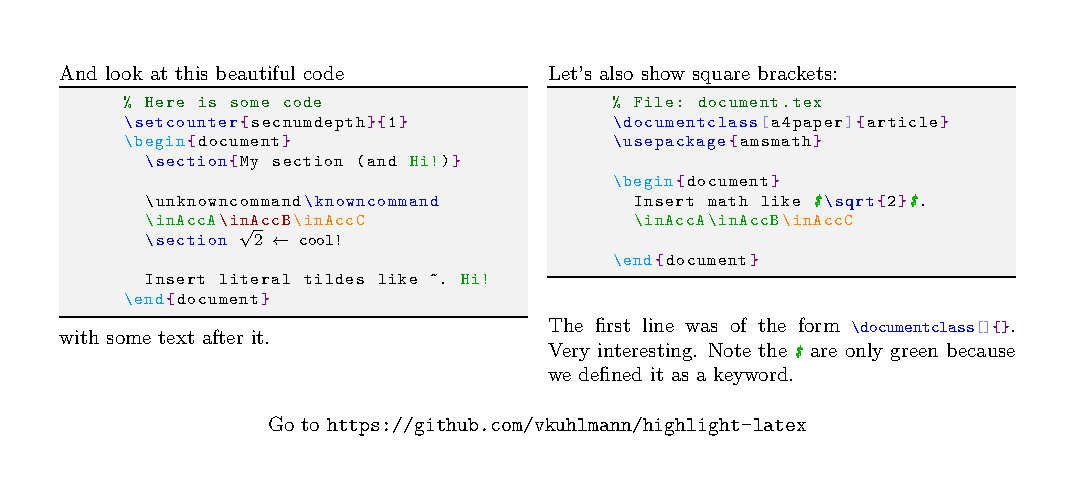
\includegraphics[width=\textwidth,trim=1cm 1cm 1cm 1cm, clip]{demo.pdf}
% 	\caption{Output of `demo.tex'.}\label{fig:demoOutput}
% 	\bigskip
% 	\rule{2cm}{1pt}
% \end{figure}
% 
% \vfil
% 
% \pagebreak
% \tableofcontents
% \pagebreak
% 
% \section{Getting started}
% 
% After having added the package, you can add LaTeX in two ways.
% 
% \subsection{Inline style}%
% 
% \begin{showcase}[label=example]%
% 	\begin{highlightblock}[gobble=3]
% 		Your file begins with a line of the form \hll~{}~|\documentclass[]{}|. The
% 		square brackets ...
% 	\end{highlightblock}%
% \end{showcase}
% 
% The first non-space character following \lstinline|\hll| delimits the argument to
% this command.
% 
% \subsection{Block style}
% 
% 
% \begin{showcase}[label=example]
% 	\begin{highlightblock}[gobble=3]
% 		Your basic document now looks like
% 		\begin{highlightblock}[gobble=2]
% 			\documentclass[a4paper]{article}
% 			\begin{document}
% 			Hello world!
% 			\end{document}
% 		\end{~{}~highlightblock}
% 	\end{highlightblock}
% \end{showcase}
% 
% To prevent indentation of our \hll|highlightblock| (here one tab) to be shown as part of the code,
% the \hll|gobble| parameter strips them off. Play around with it until everything looks right. I
% recommend to set this value globally using \hll|\def\defaultgobble{2}|. You can still override it on
% a per-block basis, if necessary.
% 
% There are situations where width of the block could run out of the page. For example, when using
% beamer and storing a block as described in the section `Fragile breaking situations', the normal
% full-width of a slide is assumed. If you use multiple columns, set the \hll|linewidth| on the
% \hll|highlightblock|. This can be a fraction of the total slide width available, \hll|0.6\textwidth|
% is 60\% of the width, or an absolute value, like \hll|10em|, which seems to equal 20 characters.
% 
% 
% There are more keys you can provide. Check the
% \fhref{https://www.ctan.org/pkg/listings}{\hll|listings| package
% 	documentation} for options
% available to the \hll|lstlisting|-environment and \hll|lstset| command.
% 
% \newbox\uphbox
% \setbox\uphbox=\hbox{\hll|\updatehighlight|}%
% \setbox\uphbox=\hbox{\adjustbox{height=1.4\height}{\usebox\uphbox}}
% 
% \section[Macro \textbackslash updatehighlight]{%
%   Macro \texorpdfstring{\usebox\uphbox}{\textbackslash updatehighlight}}
% \subsection{Adding a command to a highlighting rule}
% 
% By default, only some LaTeX commands will be highlighted in blue. If there are others you need, like
% \hll|\tableofcontents| and \hll|\figref|, update the highlighting rules:
% \begin{showcase}[label=use]
% 	\begin{highlightblock}[gobble=3]
% 		\updatehighlight{
% 			name = default,
% 			add = {
% 				\tableofcontents, \figref
% 			}
% 		}
% 	\end{highlightblock}
% \end{showcase}
% 
% The change will only affect code after it. I recommend issuing \hll|updatehighlight| in your
% preamble (before the \hll|\begin{document}|). In some situations you might want to change things
% mid-document. That's possible too.
% 
% \subsection{Custom highlighting rules}
% \subsubsection{Example}
% 
% As shown in \hll|demo.tex|, you can put any command or keyword you want to highlight in a different
% color. You do this with
% \begin{showcase}[label=example]
% 	\begin{highlightblock}[gobble=3]
% 		\updatehighlight{
% 			% The name allows you to modify the style later.
% 			name = spotlight,
% 			color = orange,
% 			add = {
% 				\tableofcontents
% 			}
% 		}
% 	\end{highlightblock}
% \end{showcase}
% 
% You can use the \hll|xcolor| syntax for describing colors as well. If you find the orange too
% bright, you can replace it with \hll|orange!90!black|: 90\% orange, remaining is black. For more
% information on color definitions and name, refer to
% \fhref{https://en.wikibooks.org/wiki/LaTeX/Colors}{LaTeX/Colors on Wikibooks}.
% 
% 
% \subsubsection{Specification}
% 
% The argument to \hll|\updatehighlight| is a key-value list. Keys are processed sequentially. For
% example, use \hll|color| before \hll|add| rather than after it, and a key can appear multiple times.
% Each one will be processed. You can merge any two \hll|\updatehighlight| in one. No need to close
% and reopen \hll|\updatehighlight| for each highlighting rule.
% 
% You might be tempted to add a blank line for clarity; that means a new paragraph to LaTeX, don't do
% it. Instead, just put a line with only a \hll|\%| sign. Spacing within the argument is often
% irrelevant. If you need a comma in the value, surround your value with braces.
% 
% 
% \begin{list}{}{%
% 		\itemindent-\leftmargin%
% 		\setlength{\itemsep}{10pt}%
% 	}
% 	\item\textbf{name}\par\nobreak
% 
% 	Creates or modifies a named rule. This key is optional.
% 
% 	The default keys are \hll|default|, which includes a bunch of basic commands, and has by default
% 	a dark blue color, and \hll|structure|, which consists of \hll|\begin| and \hll|\end| and prints
% 	them in light blue.
% 
% 
% 	\item\textbf{classoffset}\par\nobreak
% 
% 	Sets the \hll|listings| classoffset manually. Try to avoid this. Use \textbf{name} to refer to
% 	existing rules instead.
% 
% 
% 	\item\textbf{add}\par\nobreak
% 
% 	Adds a command (\hll|\mycommand|) or keyword (\hll|Hi!|) to the current rule. The value can
% 	contain multiple values by opening braces, and comma separating values within them.
% 
% 
% 	\item\textbf{remove}\par\nobreak
% 
% 	Removes a commands or keywords from the current rule. The value
% 	can contain multiple values by opening braces, and comma separating values
% 	within them.
% 
% 
% 	\item\textbf{clear}\par\nobreak
% 
% 	Removes all commands and keywords from the current rule. Use
% 	without value, for example
% 	\begin{showcase}[label=example]
% 		\begin{highlightblock}[gobble=5]
% 			\updatehighlight{
% 				name = default,
% 				clear
% 			}
% 		\end{highlightblock}
% 	\end{showcase}
% 
% 
% 	\item\textbf{color}\par\nobreak
% 
% 	Specifies a color for the rule. Equivalent to specifying \hll|style|
% 	instead, with value \hll|\color{value}| where \hll|value| is the value for the
% 	\textbf{color} key. So \hll|color=red| and \hll|style=\color{red}| are equivalent.
% 
% 
% 	\item\textbf{style}\par\nobreak
% 
% 	Specifies a style for the rule. A rule can have only one style. If
% 	you specify a style after \hll|add| or \hll|remove|, this starts a new (unnamed)
% 	rule. In practice, the only style which will probably work for you is just a
% 	color. For that, using the `color' key is just a bit easier and neater. But
% 	hey, you have the option to set whatever style you want. :)
% 
% \end{list}
% 
% \section{Global settings}
% 
% There are some global parameters involved in the appearance:
% \begin{showcase}[label=overview]
% 	\begin{highlightblock}[gobble=3]
% 		\colorlet{curlyBrackets}{red!50!blue}
% 		\colorlet{squareBrackets}{blue!50!white}
% 		\colorlet{codeBackground}{gray!10!white}
% 		\colorlet{comment}{green!40!black}
% 		\def\defaultgobble{0}
% 	\end{highlightblock}
% \end{showcase}
% 
% Each line can be set independent of each other, and each shows its default
% value.
% 
% There are package options you can use as well:
% 
% \begin{list}{}{%
% 		\itemindent-\leftmargin%
% 		\setlength{\itemsep}{10pt}%
% 	}
% 	\item\textbf{frame} (default: \hll|lines|)\par\nobreak
% 
% 	Specifies the frame you want around code. My
% 	favorites are \hll|lines| and \hll|none|. Check the
% 	\fhref{https://www.ctan.org/pkg/listings}{listings package documentation} for all
% 	possibilities.
% 
% 
% 	\item\textbf{noframe} (use without value)\par\nobreak
% 
% 	Equivalent to \hll|frame=none|.
% 
% 
% 	\item\textbf{styleanywhere} (use without value)\par\nobreak
% 
% 	Overrides the default behavior that \hll|style| starts a new style after commands like \hll|add| and \hll|remove|.
% 
% \end{list}
% 
% 
% \section{Fragile breaking situations (like beamer frames)}
% 
% When passing command arguments around, or storing environment content, LaTeX interprets all
% characters. This includes seeing \hll|\maketitle| in \hll!\hll|\maketitle|! as a real command. To
% prevent this behavior, everything from \hll|\verb|, \iffalse|\fi to the \hll|verbatim|-environment,
% to the \hll|listings| package (which this package depends on) temporarily changes the interpretation
% of characters that are still to be read. The blackslash before maketitle in \hll!\hll|\maketitle|!
% will be read as `just text' (a \textit{letter} technically).
% 
% When content has already been interpreted, like the \hll|frame|-environment in \hll|beamer| does,
% this trick can't be done anymore. Instead, you either need to \emph{escape} code, or
% \emph{pre-process} the code outside a fragile breaking situation.
% 
% Escaping is done by preceding the special character with a backslash. For example,
% \hll!\hll|\documentclass[]{}|! becomes \hll!\hll|\\!\hll!documentclass[]\{\}|!.
% 
% For large code blocks, this is undesirable. Therefore, the package provides for a companion to the
% \hll|highlightblock|-environment: surround it with a \hll|saveblock|-environment which takes a
% single argument: a name to assign it. We use it to refer to it later. For example:
% \begin{showcase}[label=example]
% 	\begin{highlightblock}[gobble=3]
% 		\begin{saveblock}{basicfigure}
% 			\begin{highlightblock}[linewidth=0.6\textwidth]
% 				\begin{figure}
% 					\includegraphics
% 					[width=0.9\linewidth]
% 					{myPlot.pdf}
% 
% 					\caption{My plot}
% 					\label{fig:myplot}
% 				\end{figure}
% 			\end{highlightblock~{}~}
% 		\end{saveblock}
% 	\end{highlightblock}
% \end{showcase}
% 
% 
% Do this outside a fragile breaking situation. (For the \hll|frame|-environment example, that means
% just before the \hll|frame| for example.) Then, where you want to use it, use
% \hll|\useblock{basicfigure}|. There is also a variant \hll|\consumeblock{basicfigure}|. If you save
% many blocks, these will all remain loaded in memory till your PDF has fully generated. The
% \hll|\consumeblock| works like \hll|\useblock|, except the saved block is deleted from memory after
% its use. Note this can also result in unexpected behavior, for example animations in a beamer frame
% might need the code line to be executed multiple times. Use \hll|\useblock| when you can't make the
% guarantee the last use of a block.
% 
% There is a separate demo for fragile breaking situations. You can find it at
% \hll|deamerdemo/deamerdemo.tex|.
% 
% \section{Adding extra space}
% 
% By default, highlight-latex follows an approach where it minimizes spacing. This gives you full
% control over how tight or spacious your document looks. Just use commands like \hll|\medskip| to add
% extra spacing. The package doesn't currently include an option to do it everywhere automatically.
% 
% \section{License}
% 
% The package is available under MIT License. See \textsc{license}.txt.
% 
% \section{Credits}
% 
% Thanks for minor fixes:
% 
% gemmaro
% 
% \rule{5cm}{0.4pt}
% 
% For any bug, feature request, unclarity, or whatever else related to this package, you're welcome to
% open an issue or pull-request. Issues can be opened on
% 
% \begin{showcase}[label=url]
% 	\begin{highlightblock}[gobble=3]
% 		~\url{https://github.com/vkuhlmann/highlight-latex/issues}~
% 	\end{highlightblock}
% \end{showcase}
% 
% Thanks for contributing!
% 
% 
% 
%
% \section{Implementation}
%
%    \begin{macrocode}
\NeedsTeXFormat{LaTeX2e}[1994/06/01]
\ProvidesPackage{highlightlatex}[2021/03/17 highlightlatex v1.0.0 + Dev]

% Repository: https://github.com/vkuhlmann/highlight-latex
% Version: v1.0.0 + Dev

% Copyright (c) 2021 Vincent Kuhlmann
% 
% Permission is hereby granted, free of charge, to any person
% obtaining a copy of this software and associated documentation
% files (the "Software"), to deal in the Software without
% restriction, including without limitation the rights to use,
% copy, modify, merge, publish, distribute, sublicense, and/or sell
% copies of the Software, and to permit persons to whom the
% Software is furnished to do so, subject to the following
% conditions:
% 
% The above copyright notice and this permission notice shall be
% included in all copies or substantial portions of the Software.
% 
% THE SOFTWARE IS PROVIDED "AS IS", WITHOUT WARRANTY OF ANY KIND,
% EXPRESS OR IMPLIED, INCLUDING BUT NOT LIMITED TO THE WARRANTIES
% OF MERCHANTABILITY, FITNESS FOR A PARTICULAR PURPOSE AND
% NONINFRINGEMENT. IN NO EVENT SHALL THE AUTHORS OR COPYRIGHT
% HOLDERS BE LIABLE FOR ANY CLAIM, DAMAGES OR OTHER LIABILITY,
% WHETHER IN AN ACTION OF CONTRACT, TORT OR OTHERWISE, ARISING
% FROM, OUT OF OR IN CONNECTION WITH THE SOFTWARE OR THE USE OR
% OTHER DEALINGS IN THE SOFTWARE.

\RequirePackage{listings}
\RequirePackage{xcolor}

\RequirePackage{xkeyval}
\RequirePackage{etoolbox}

%% Snippet source:
%% https://tex.stackexchange.com/questions/406015/defining-macro-gsetlength-as-global-setlength-reliable
\gdef\gsetlength#1#2{%
  \begingroup
    \setlength\skip@{#2}%
    \global#1=\skip@
  \endgroup
}


\def\@highlight@frame{none}
\newlength{\hll@offset@fixskip}
\setlength{\hll@offset@fixskip}{0pt}

\newif\ifhllStyleAnywhere
\newcommand\defaultgobble{0}
\newif\ifhllDebugFrame
%\hllDebugFrametrue
\newlength\hllBeforeSkip
\setlength\hllBeforeSkip{2pt}
\newlength\hllAfterSkip
\setlength\hllAfterSkip{0pt}

%    \end{macrocode}
% \subsection{Package options}

%    \begin{macrocode}
\DeclareOptionX{frame}{
  \setframe{#1}
}

\DeclareOptionX{noframe}{
  \setframe{none}
}

\def\setframe#1{%
  \def\frameval{#1}%
  \ifx\relax#1\relax
    \def\frameval{lines}%
  \fi
  \def\linesvalue{lines}%
  %
  \xdef\@highlight@frame{\frameval}%
  %
  \ifx\frameval\linesvalue
    \gsetlength{\hll@offset@fixskip}{6pt}%
  \else
    \gsetlength{\hll@offset@fixskip}{0pt}%
  \fi
}

\DeclareOptionX{styleanywhere}{
  \hllStyleAnywheretrue
}

\DeclareOptionX*{\PackageWarning{highlightlatex}{`\CurrentOption' ignored}}
\ExecuteOptionsX{frame=lines}

\ProcessOptionsX\relax

%    \end{macrocode}
% \subsection{Initialization}

%    \begin{macrocode}
\colorlet{curlyBrackets}{red!50!blue}
\colorlet{squareBrackets}{blue!50!white}
\colorlet{codeBackground}{gray!10!white}
\colorlet{comment}{green!40!black}

\colorlet{accDefault}{blue!90!black}
\definecolor{accStructure}{RGB}{0,149,255}

\colorlet{accentB}{green!60!black}

\catcode`\{=11
\let\myopenbrace={
\catcode`\{=1

\catcode`\}=11
\let\myclosebrace=}
\catcode`\}=2

\lstdefinelanguage{ColoredLaTeX}
[LaTeX]{TeX}{
  backgroundcolor=\color{codeBackground},
  keywordstyle=\bfseries\color{accDefault},
  basicstyle=\footnotesize\ttfamily,
  commentstyle=\color{comment},
  numbers=none,
  tabsize=2,
  mathescape=false,
  alsoletter={$@_!|?$},
%
  classoffset=0,
  keywordstyle=\color{accDefault},
  texcsstyle=*\color{accDefault},
  moretexcs={subsection,thesubsection,thesection,theoremstyle},
  deletetexcs={begin,end},
%
  classoffset=1,
  keywordstyle=\color{accStructure},
  texcsstyle=*\color{accStructure},
  moretexcs={begin,end},
%
  classoffset=2,
  escapeinside=~~,
%  
  classoffset=0,
  %literate={textA}{textB}{3}%
  %https://tex.stackexchange.com/questions/172945/coloring-in-listing
  literate={\{}{{\textcolor{curlyBrackets}{\myopenbrace}}}{1}
    {\}}{{\textcolor{curlyBrackets}{\myclosebrace}}}{1}
    {[}{{\textcolor{squareBrackets}{[}}}{1}
    {]}{{\textcolor{squareBrackets}{]}}}{1}%
  %    {(}{{\textcolor{delimiterColor}{(}}}{1}
  %    {)}{{\textcolor{delimiterColor}{)}}}{1}%
  %texcsstyle=\color{blue}
}
\lstset{language=ColoredLaTeX}

\def\hll@assignlabel#1#2{%
  \expandafter\gdef\csname hll@labeltoclassoffset@#1\endcsname{#2}%
}

\hll@assignlabel{default}{0}
\hll@assignlabel{structure}{1}

%    \end{macrocode}
% \subsection{Options}
%    \begin{macrocode}

\newcommand{\hllDelimDollar}[1][\color{green!40!black}]{%
  \lstset{
    classoffset=2,
    moredelim=**[s][#1]{$}{$},
    classoffset=0
  }%
}

\newcommand{\hllDelimParen}[1][\color{green!40!black}]{%
  \lstset{
    classoffset=2,
    moredelim=**[s][#1]{\(}{\)},
    classoffset=0
  }%
}

%    \end{macrocode}
% \subsection{Block and inline markup}
%    \begin{macrocode}


\newcommand{\hllPrepareBlock}{%
  \lstset{framesep=0.1cm,framerule=0.6pt}%
  \def\setHighlightFrame##1{%
    \lstset{frame=##1}%
  }%
  \expandafter\setHighlightFrame\expandafter{\@highlight@frame}%
  \lstset{belowskip=0pt,aboveskip=0pt,belowcaptionskip=0pt,gobble=\defaultgobble}%
  \setlength\parskip{0pt}%
  \setlength\parindent{0pt}%
}

\lstnewenvironment{highlightblock}[1][]
{%
  \vspace{\hllBeforeSkip}%
  \begingroup
  \hllPrepareBlock\lstset{#1}%
}{%
  \nointerlineskip
  \endgroup
  \vspace{\hllAfterSkip}%
}

\lstnewenvironment{hllblock}[1][]
{%
  \vspace{\hllBeforeSkip}%
  \begingroup
  \hllPrepareBlock\lstset{#1}%
}{%
  \endgroup
  \vspace{\hllAfterSkip}%
}

\def\hll{\lstinline}

%    \end{macrocode}
% \subsection{Block saving}


%    \begin{macrocode}


\newenvironment{saveblock}[1]{%
  \expandafter\ifx\csname @codebox@#1\endcsname\relax
    \expandafter\newbox\csname @codebox@#1\endcsname\relax
  \fi
  %
  %% The trick from latex/base/latex.ltx
  \edef\@bracehack{%
    \endgroup
    \expandafter\setbox\csname @codebox@#1\endcsname\vbox{%
      \begingroup\aftergroup}%
    \def\noexpand\@currenvir{\@currenvir}%
    \def\noexpand\@currenvline{\on@line}}%
  \@bracehack
  \begingroup\vspace{\hll@offset@fixskip}
  \ignorespaces%
}{%
  \endgroup
}

\newcommand\useblock[1]{%
  \ifhllDebugFrame
    \par
    {%
      \setlength{\fboxsep}{0pt}%
      \fcolorbox{orange}{red}{\expandafter\usebox\csname @codebox@#1\endcsname}%
    }%
    \par
  \else
    \par\expandafter\usebox\csname @codebox@#1\endcsname\par
  \fi
}

\newcommand\consumeblock[1]{%
  \ifhllDebugFrame
    \par
    {%
      \setlength{\fboxsep}{0pt}%
      \setlength{\fboxrule}{1pt}%
      \fcolorbox{orange}{red}{\leavevmode\expandafter\box\csname @codebox@#1\endcsname\relax}%
    }
    \par
    \expandafter\let\csname @codebox@#1\endcsname\relax
  \else
    \par\leavevmode\expandafter\box\csname @codebox@#1\endcsname\relax\par
    \expandafter\let\csname @codebox@#1\endcsname\relax
  \fi
}

%    \end{macrocode}
% \subsection{Macro \textbackslash updatehighlight}


%    \begin{macrocode}
\def\hll@update@label{}

\newcounter{hll@update@state}

\newcounter{hll@update@nextclassoffset}
\setcounter{hll@update@nextclassoffset}{5}

\newcounter{hll@update@classoffset}

\def\hll@update@fixclassoffset{%
  \ifnum\value{hll@update@state}<1\relax
  \setcounter{hll@update@classoffset}{\thehll@update@nextclassoffset}%
  \stepcounter{hll@update@nextclassoffset}%
  \setcounter{hll@update@state}{1}%
  \fi
}

\newcommand{\updatehighlight}[1]{%
  \setcounter{hll@update@state}{-1}%
  \gdef\hll@update@label{}%
  \setkeys{updatehighlight}{#1}%
  %
  \lstset{classoffset=0}%
}

%    \end{macrocode}
% \subsubsection{Key `name'}


%    \begin{macrocode}
\define@key{updatehighlight}{name}{%
  \hll@update@setlabel{#1}%
}

\def\hll@update@setlabel#1{
  \gdef\hll@update@label{#1}%
  \expandafter\def\expandafter\@capturedlabel\expandafter{\csname hll@labeltoclassoffset@#1\endcsname}%
  \expandafter\unless\expandafter\ifx\@capturedlabel\relax\relax
    % Label exists
    \edef\@val{\@capturedlabel}%
    \setcounter{hll@update@classoffset}{\@val}%
    \setcounter{hll@update@state}{1}%
  \else
    % Allocate new label
    \edef\@val{\thehll@update@nextclassoffset}%
    \setcounter{hll@update@classoffset}{\@val}%
    \stepcounter{hll@update@nextclassoffset}%
    \setcounter{hll@update@state}{1}%
    %
    \expandafter\xdef\@capturedlabel{\@val}%
  \fi
}

%    \end{macrocode}
% \subsubsection{Key `classoffset'}


%    \begin{highlightblock}[numbers=left,firstnumber=last]
% ~{\makeatletter\meaning\lstenv@endstring\expandafter\def\expandafter\lstenv@endstring\expandafter{\lstenv@endstring a}}~
\define@key{updatehighlight}{classoffset}{%
  \setcounter{hll@update@classoffset}{#1}%
  \setcounter{hll@update@state}{1}%
}
% tadaaa
% \end{highlightblock}aaa
% \subsubsection{Key `add'}


%    \begin{macrocode}
\define@key{updatehighlight}{add}{%
  \hll@update@add{#1}%
}

\def\hll@update@add#1{%
  \hll@update@fixclassoffset
  \def\@inv##1{\forcsvlist{\hll@update@additem{##1}}{#1}}%
  \expandafter\@inv\expandafter{\the\c@hll@update@classoffset}
  %
  \setcounter{hll@update@state}{2}%
}

\def\hll@update@additem#1#2{%
  \if\noexpand#2\relax
    \edef\keywordpure{\expandafter\@gobble\string#2}%
    \def\callwithpure##1{\hll@update@addmacro{#1}{##1}}%
    \expandafter\callwithpure\expandafter{\keywordpure}%
  \else
    \hll@update@addkeyword{#1}{#2}%
  \fi
}

\def\hll@update@addmacro#1#2{%
  \lstset{
    classoffset=0,deletetexcs={#2},
    classoffset=1,deletetexcs={#2},
    classoffset=#1,moretexcs={#2},
    classoffset=0
  }%
}

\def\hll@update@addkeyword#1#2{%
  \lstset{
    classoffset=0,deletekeywords={#2},
    classoffset=1,deletekeywords={#2},
    classoffset={#1},otherkeywords={#2},morekeywords={#2},
    classoffset=0
  }%
}

%    \end{macrocode}
% \subsubsection{Key `remove'}


%    \begin{macrocode}
\define@key{updatehighlight}{remove}{%
  \hll@update@remove{#1}%
}

\def\hll@update@remove#1{%
  \hll@update@fixclassoffset
  \def\@inv##1{\forcsvlist{\hll@update@removeitem{##1}}{#1}}%
  \expandafter\@inv\expandafter{\the\c@hll@update@classoffset}
  %
  \setcounter{hll@update@state}{2}%
}

\def\hll@update@removeitem#1#2{%
  \if\noexpand#2\relax
    \edef\keywordpure{\expandafter\@gobble\string#2}%
    \def\callwithpure##1{\hll@update@removemacro{#1}{##1}}%
    \expandafter\callwithpure\expandafter{\keywordpure}%
  \else
    \hll@update@removekeyword{#1}{#2}%
  \fi
}

\def\hll@update@removemacro#1#2{%
  \lstset{
    classoffset={#1},
    deletetexcs={#2},
    classoffset=0
  }%
}

\def\hll@update@removekeyword#1#2{%
  \lstset{
    classoffset={#1},
    deletekeywords={#2},
    classoffset=0
  }%
}

%    \end{macrocode}
% \subsubsection{Key `style'}


%    \begin{macrocode}
\define@key{updatehighlight}{style}{%
  \hll@update@fixclassoffset
  \unless\ifhllStyleAnywhere
    \ifnum\value{hll@update@state}>1\relax
      \setcounter{hll@update@state}{0}%
      \hll@update@fixclassoffset
    \fi
  \fi
  %
  \expandafter\hll@update@setstyle\expandafter{\the\c@hll@update@classoffset}{#1}%
}

\def\hll@update@setstyle#1#2{%
  \lstset{%
    classoffset={#1},
    keywordstyle={#2},
    texcsstyle={*#2},
  }%
}

%    \end{macrocode}
% \subsubsection{Key `color'}


%    \begin{macrocode}
\define@key{updatehighlight}{color}{%
  \hll@update@fixclassoffset
  \unless\ifhllStyleAnywhere
    \ifnum\value{hll@update@state}>1\relax
      \setcounter{hll@update@state}{0}%
      \hll@update@fixclassoffset
    \fi
  \fi
  %
  \expandafter\hll@update@setcolor\expandafter{\the\c@hll@update@classoffset}{#1}%
}

\def\hll@update@setcolor#1#2{%
  \lstset{%
    classoffset={#1},
    keywordstyle={\color{#2}},
    texcsstyle={*\color{#2}},
  }%
}

%    \end{macrocode}
% \subsubsection{Key `clear'}


%    \begin{macrocode}
\define@key{updatehighlight}{clear}[]{%
  \hll@update@fixclassoffset
  \expandafter\hll@update@clear\expandafter{\the\c@hll@update@classoffset}%
}

\def\hll@update@clear#1{%
  \lstset{
    classoffset={#1},
    texcs={},
    keywords={},
    classoffset=0
  }%
}
%    \end{macrocode}
%
% \Finale
%
\endinput
